\documentclass[10pt]{exam}
\usepackage[hon]{template-for-exam}
\usepackage{tikz}
\usetikzlibrary{
  calc,
  patterns,
  decorations.pathmorphing,
}





\title{Energy in Simple Harmonic Oscillators}
\author{Rohrbach}
\date{\today}

\begin{document}
\maketitle

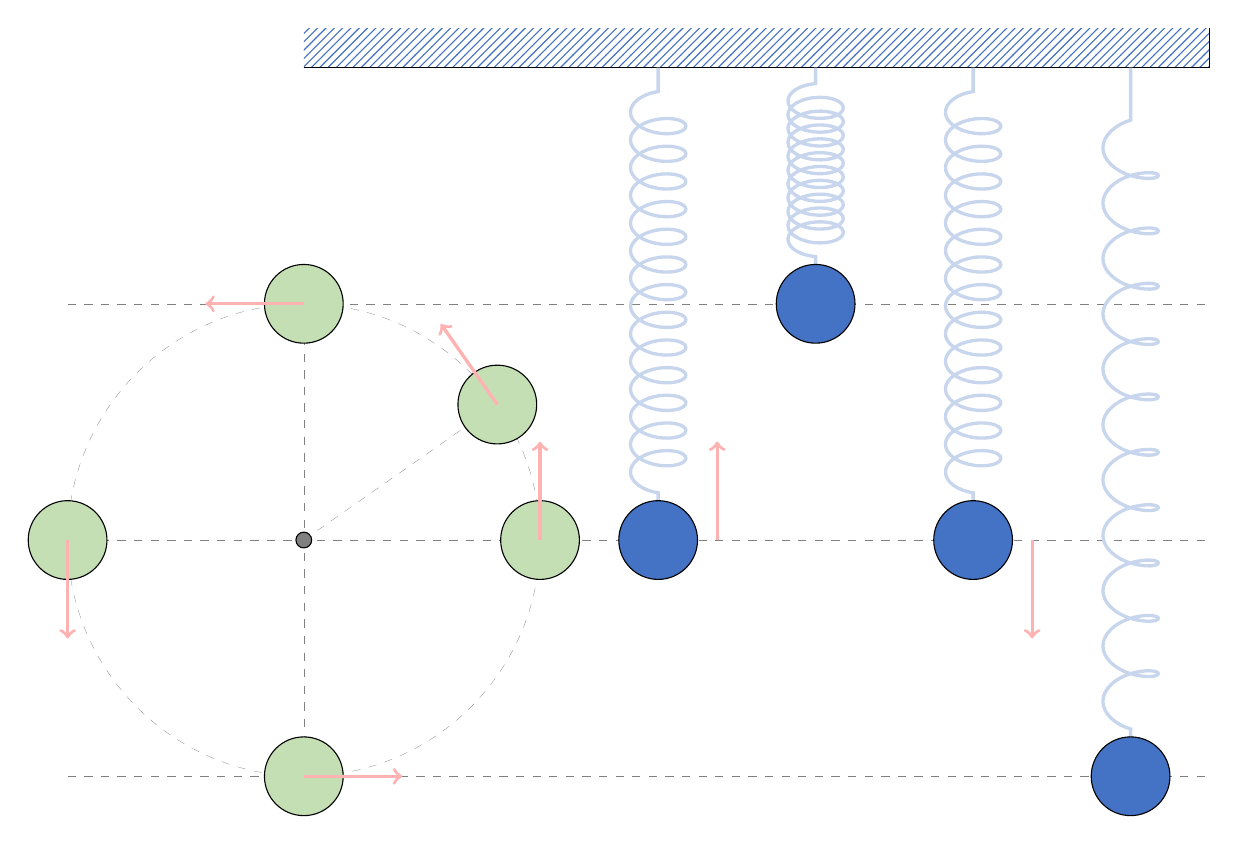
\begin{tikzpicture}
  \def\amp{3}
  \def\massradius{.5}
  \def\sep{2}
  \def\ceilingheight{2*\amp}
  \def\startofspring{\amp+1.5}
  \def\endofpicx{\startofspring+3.5*\sep}
  \def\springending{.1}
  \def\veclength{1.25}

  \definecolor{springcolor}{HTML}{4472C4}
  \definecolor{circlecolor}{HTML}{C5DFB5}

  \tikzstyle{guides}=[
      ultra thin,
      gray,
      dashed
    ]
  \tikzstyle{cmass}=[
      radius=\massradius,
      fill=circlecolor
    ]
  \tikzstyle{smass}=[
      radius=\massradius,
      fill=springcolor,
    ]
  \tikzstyle{ceiling}=[
      pattern=north east lines,
      pattern color=springcolor
    ]
  \tikzstyle{spring}=[
      very thick,
      springcolor!30,
      decoration={
        coil,
        amplitude=10
      }
    ]
  \tikzstyle{vector}=[
      red!30,
      very thick,
      ->
    ]

  \coordinate (ceiling start) 
                  at (0, \ceilingheight);
  \coordinate (ceiling end)   
                  at (\endofpicx, \ceilingheight);
  \fill[ceiling] (ceiling start) -- (ceiling end)
     -- ++(0,.5) -- ++ ($-1*(\endofpicx ,0)$) -- cycle;
  \draw (ceiling start) -- (ceiling end) -- ++ (0,.5);

  \draw[guides] (-\amp,  0  ) -- (\endofpicx,    0 );
  \draw[guides] (-\amp, \amp) -- (\endofpicx,  \amp);
  \draw[guides] (-\amp,-\amp) -- (\endofpicx, -\amp);
  \draw[guides] (0    , \amp) -- (0         , -\amp);

  \coordinate (ccenter) at (0,0);
  \filldraw[fill=gray] (ccenter) circle[radius=0.1];
  \draw[guides]        (ccenter) circle[radius=\amp];


  \coordinate (c1) at (  0:\amp);
  \coordinate (c2) at ( 35:\amp);
  \coordinate (c3) at ( 90:\amp);
  \coordinate (c4) at (180:\amp);
  \coordinate (c5) at (270:\amp);
  
  \draw[guides] (ccenter) -- (c2);

  \foreach \x in {(c1),(c2),(c3),(c4),(c5)} {
    \draw[cmass] \x circle;
  }

  \draw[vector] (c1) -- ++( 90:\veclength);
  \draw[vector] (c2) -- ++(125:\veclength);
  \draw[vector] (c3) -- ++(180:\veclength);
  \draw[vector] (c4) -- ++(270:\veclength);
  \draw[vector] (c5) -- ++(  0:\veclength);



  \path[smass] (ccenter) 
    ++(\startofspring,  0 ) coordinate (s1)
    ++(\sep,          \amp) coordinate (s3)
    ++(\sep,         -\amp) coordinate (s4)
    ++(\sep,         -\amp) coordinate (s5);


  %usage \drawspring{(location of mass)}{segment length}
  \newcommand{\drawspring}[2]{
    \coordinate (thismass) at #1;
    \coordinate (top) at 
      ($(ceiling start)!(thismass)!(ceiling end)$);
    \draw[spring,segment length=#2] (thismass)
      -- ++ (0,\massradius+\springending) 
      decorate {-- ($(top) + (0,-\springending)$) }
      -- (top);
  }

  \drawspring{(s1)}{10}
  \draw[smass] (s1) circle;
  \draw[vector] ($(s1)+(1.5*\massradius,0)$) 
    -- ++ (0,\veclength);

  \drawspring{(s3)}{5}
  \draw[smass] (s3) circle;

  \drawspring{(s4)}{10}
  \draw[smass] (s4) circle;
  \draw[vector] ($(s4)+(1.5*\massradius,0)$)  
    -- ++ (0,-\veclength);

  \drawspring{(s5)}{20}
  \draw[smass] (s5) circle;


\end{tikzpicture}

\pagebreak

\section*{Practice}

%\begin{questions}

%\question
  A 0.60-kg mass is placed on a spring and set to oscillate with an amplitude of 13~cm.  Its frequency is 4.0~Hz.

  \vspace{1em}

  \begin{parts}
    \part
      Calculate the maximum speed of the mass.
    \part
      How fast is the mass moving when its displacement from equilibrium is 9~cm?
    \part
      Write down the equation for motion of the mass.
  \end{parts}

  \vs[3]

% \question 
%   An object of mass 0.75~kg oscillates according to the equation $x(t)=0.45\cos\left(6.40 \cdot t\right)$, where $x$ is measured in meters and $t$ is measured in seconds.


%   \begin{parts}
%     \part
%       What is the amplitude?
%     \part
%       What is the frequency?
%     \part
%       What is the total energy of the system?
%   \end{parts}

%   \vs



  
% \end{questions}



\end{document}